\documentclass[11pt,a4paper]{article}
\usepackage[czech]{babel}
\usepackage[utf8]{inputenc}
\usepackage[T1]{fontenc}
\usepackage[left=2.5cm,right=2.5cm,top=2.5cm,bottom=2.5cm]{geometry}
\usepackage{graphicx}
\usepackage{pdfpages}
\usepackage{booktabs}
\usepackage{longtable}
\usepackage{pdflscape}
\newcommand{\T}[1]{\texttt{#1}}
\usepackage{xcolor}
\usepackage{tikz}
\usetikzlibrary{positioning,arrows.meta}
\usepackage[hidelinks]{hyperref}


\newcommand{\doplnit}[1]{\textcolor{red}{[DOPLNIT: #1]}}

\begin{document}

\begin{titlepage}
  \centering
  
\includegraphics[width=0.7\textwidth]{logo_fit.png}

  \vspace{3cm}
  {\Huge\bfseries Projektová dokumentace\par}
  \vspace{0.8cm}
  {\LARGE Implementace překladače jazyka IFJ26\par}
  \vspace{0.4cm}
  {\Large Tým xstrelm00, varianta TRP-izp\par}

  \vspace{2cm}
  {\large
  \renewcommand{\arraystretch}{1.6}
  \setlength{\tabcolsep}{10pt}
  \begin{tabular}{llll}
    \textit{Řešitel} & \textit{Login} & \textit{Osobní číslo} & \textit{Body} \\
    \textbf{Maksym Streltsov (vedoucí)} & \textbf{xstrelm00} & \textbf{281996} & \textbf{25\,\%} \\
    Yaryna Kotliarenko  & xkotliy00 & 274157 & 25\,\% \\
    Jakub Šmíd          & xsmidja00 & 260102 & 25\,\% \\
    Tamerlan Alimzhanov & xalimzt00 & 282142 & 25\,\% \\
  \end{tabular}
  \par}

  \vspace{1.5cm}
  {\large Rozšíření: BOOLTHEN, CONTROL, FUNEXP, PARAMLISTS, VALMEM\par}
  \vspace{0.4cm}
  {\large Repozitář: \url{https://github.com/tmrln1112/IFJ-project}\par}

  \vfill
  {\Large 27. listopadu 2026\par}
\end{titlepage}
\tableofcontents
\newpage
\section{Úvod}
Překladač implementuje celé základní zadání a rozšíření BOOLTHEN, CONTROL,
FUNEXP, PARAMLISTS a VALMEM. 


\section{Práce v~týmu}

\subsection{Rozdělení práce}
\begin{itemize}
 \item \textbf{Maksym Streltsov} -- sémantická analýza, tabulka symbolů,
        globální testy překladače.
  \item \textbf{Yaryna Kotliarenko} -- lexikální analyzátor a jeho testy,
        diagram konečného automatu, kontrola rozšíření podle specifikace,
        dokumentace.
  \item \textbf{Jakub Šmíd} -- syntaktický analyzátor (rekurzivní sestup,
        precedenční analýza výrazů), LL gramatika, LL a precedenční tabulka.
  \item \textbf{Tamerlan Alimzhanov} -- generátor cílového kódu IFJcode26
        a vestavěné funkce, prezentace k~obhajobě.
\end{itemize}
Body jsou rozděleny rovnoměrně, všichni členové se na projektu podíleli
srovnatelným dílem.


\subsection{Spolupráce, testování a styl kódu}
\begin{itemize}
  \item Kód máme v~soukromém repozitáři na GitHubu. Každou změnu děláme
        ve vlastní větvi a do \texttt{main} ji dostaneme přes pull request.
        Commity pojmenováváme podle Conventional Commits
        (např. \texttt{fix(scanner): \dots}).
  \item Každý pull request si před sloučením projde a schválí aspoň jeden
        další člen týmu, sloučí ho pak autor. Komunikujeme přes Discord,
        větší změny, které se týkají více modulů, řešíme společně na hovoru.
  \item Skener má vlastní testy (\texttt{tests/scanner}, \texttt{make test}):
        u~správných vstupů porovnáváme vypsané tokeny s~očekávanými,
        chybné vstupy musí skončit kódem~1. Celý překladač testujeme
        v~\texttt{tests/global} na správných programech i na programech
        s~chybou a kontrolujeme návratový kód, s~interpretem i výstup.
        Když opravíme chybu, přidáme na ni test.
  \item Kód formátujeme nástrojem \texttt{clang-format} ve stylu LLVM
        (\texttt{make format}).
\end{itemize}

\section{Architektura překladače}

\begin{figure}[h]
\centering
\begin{tikzpicture}[
  box/.style={draw, rounded corners, minimum width=2.7cm, minimum height=1.1cm,
              align=center, font=\small},
  aux/.style={draw, dashed, rounded corners, minimum width=2.4cm,
              minimum height=0.9cm, align=center, font=\small},
  io/.style={font=\small\itshape, align=center},
  arr/.style={-{Stealth[length=2mm]}, thick},
  lab/.style={font=\scriptsize, align=center}]
  \node[io]                        (in)   {zdrojový kód\\(\texttt{stdin})};
  \node[box, right=0.9cm of in]    (scan) {Lexikální analýza\\\texttt{scanner.c}};
  \node[box, right=2.6cm of scan]  (pars) {Syntaktická analýza\\\texttt{parser.c}};
  \node[aux, right=0.9cm of pars]  (ps)   {Zásobník\\\texttt{pstack.c}};
  \node[box, below=1.9cm of pars]  (sem)  {Sémantická analýza\\\texttt{semantic.c}};
  \node[aux, right=0.9cm of sem]   (st)   {Tabulka symbolů\\\texttt{symtable.c}};
  \node[box, left=2.6cm of sem]    (gen)  {Generátor kódu\\\texttt{codegen.c}};
  \node[io, left=0.9cm of gen]     (out)  {IFJcode26\\(\texttt{stdout})};

  \draw[arr] (in) -- (scan);
  \draw[arr] (scan) -- node[lab, above] {\texttt{Token}} node[lab, below] {\texttt{get\_token()}} (pars);
  \draw[arr, <->] (pars) -- node[lab, above] {výraz} (ps);
  \draw[arr] (pars) -- node[lab, right] {AST\\(\texttt{ast\_node})} (sem);
  \draw[arr] (sem) -- node[lab, below] {AST s~anotacemi} (gen);
  \draw[arr, <->] (sem) -- (st);
  \draw[arr] (gen) -- (out);
\end{tikzpicture}
\caption{Moduly překladače a datové toky mezi nimi (čárkovaně pomocné
datové struktury)}
\end{figure}
Parser si od skeneru bere tokeny postupně funkcí
\texttt{get\_token()} a staví z~nich abstraktní syntaktický strom
(\texttt{ast\_node}). Výrazy zpracovává precedenční analýzou se zásobníkem
z~modulu \texttt{pstack}. Hotový strom předá \texttt{main.c} sémantické
analýze. Ta si ho převede do vlastní podoby (\texttt{ASTNode}),
zkontroluje ho pomocí tabulky symbolů a do původního stromu doplní
informace pro generátor, např. kde je potřeba převést \texttt{Int}
na \texttt{Double}. Generátor pak ze stromu vypíše program v~IFJcode26
na standardní výstup. Pokud některá část najde chybu, překlad skončí
s~odpovídajícím návratovým kódem.


\section{Návrh a implementace}

\subsection{Lexikální analýza}

Lexikální analyzátor (\texttt{scanner.c}) je deterministický konečný automat.
Aktuální stav drží proměnná typu \texttt{State}; každému nekoncovému uzlu
diagramu v~příloze~\ref{app:fsm} odpovídá jedna hodnota tohoto výčtu
a v~komentáři u~ní je uveden název uzlu z~diagramu. Parser volá funkci
\texttt{get\_token()}, která čte vstup po znacích, prochází automatem a při
každém volání vrátí jeden token. Text lexému se během čtení ukládá do
dynamického řetězce (\texttt{dynstr}), takže délka identifikátorů ani
řetězců není omezena.

\paragraph{Rozhraní s~parserem.}
Token (\texttt{Token}) obsahuje typ, atribut (řetězec nebo \texttt{NULL}),
číslo řádku a příznak \texttt{newline\_before} (viz níže). Atribut mají jen
identifikátory a literály:
\begin{itemize}

  \item číselný literál zůstává jako text, jen bez podtržítek a bez přípony
        \texttt{d}/\texttt{D}; na číslo ho převádějí až další části překladače,
  \item u~řetězcového literálu jsou escape sekvence už nahrazeny skutečnými
        znaky,
  \item klíčové slovo se pozná až po načtení celého identifikátoru, a to
        vyhledáním v~tabulce klíčových slov; rezervována jsou i klíčová slova
        rozšíření.
\end{itemize}
Například řádek \texttt{val x = 3.5} skener rozloží na tokeny
\texttt{T\_VAL}, \texttt{T\_ID}\,(\texttt{x}), \texttt{T\_ASSIGN},
\texttt{T\_LIT\_DOUBLE}\,(\texttt{3.5}) a \texttt{T\_EOL};
v~závorce je uveden atribut.

Samotné podtržítko, samotné \texttt{|} a hranaté závorky \texttt{[},
\texttt{]} jsou ve specifikaci určeny pro rozšíření. Skener je vrací jako
tokeny (\texttt{T\_UNDERSCORE}, \texttt{T\_PIPE}, \texttt{T\_LBRACKET},
\texttt{T\_RBRACKET}) a jejich nepovolené použití odhalí parser jako
syntaktickou chybu. Paměť atributu uvolňuje ten, kdo token převzal, funkcí
\texttt{free\_token()}. Po posledním tokenu (i po chybě) se volá
\texttt{scanner\_free()}, která uvolní zásobník odsazení.

\paragraph{Odsazení a konce řádků.}
Na konci každého neprázdného řádku vrátí skener token \texttt{T\_EOL}.
Na začátku dalšího řádku spočítá mezery a porovná je s~úrovní aktuálního
bloku (vrchol zásobníku odsazení):
\begin{itemize}
  \item stejné odsazení -- pokračuje se ve stejném bloku,
  \item větší odsazení -- začíná nový blok, skener vrátí \texttt{T\_INDENT}
        a novou úroveň uloží na zásobník,
  \item menší odsazení -- končí jeden nebo více bloků, skener vrací
        \texttt{T\_DEDENT} (při každém volání jeden), dokud se nedostane na
        stejnou úroveň. Pokud taková úroveň na zásobníku není (odsazení
        padne mezi dvě uložené úrovně), jde o~lexikální chybu.
\end{itemize}
Tabulátor v~odsazení je lexikální chyba. Prázdné řádky a řádky jen
s~komentářem odsazení neovlivňují. Na konci souboru skener vrátí
\texttt{T\_EOL} (i když poslední řádek nekončí znakem konce řádku),
potom \texttt{T\_DEDENT} pro každý ještě otevřený blok a nakonec
\texttt{T\_EOF}.

Uvnitř kulatých závorek se konec řádku bere jako mezera, takže výraz nebo
seznam argumentů může pokračovat na dalším řádku. Takový řádek musí být
odsazen víc než začátek příkazu; jen uzavírací \texttt{)} smí být na stejné
úrovni. Pokud byl uvnitř závorek před tokenem přeskočen konec řádku, má
token nastaven příznak \texttt{newline\_before}. Podle něj parser pozná,
zda je povolena čárka před \texttt{)}.

\paragraph{Odchylky od konečného automatu.}
Kromě aktuálního stavu si skener pamatuje ještě několik údajů, které čistý
konečný automat nemá:
\begin{itemize}
  \item \textbf{zásobník odsazení} -- pamatuje si úrovně odsazení
        otevřených bloků, aby skener poznal, kdy vrátit \texttt{T\_INDENT}
        a kolik \texttt{T\_DEDENT}; podle potřeby se zvětšuje,
  \item \textbf{hloubku vnoření komentářů} $h$ -- blokové komentáře lze
        vnořovat, a komentář tak končí až u~posledního \texttt{*/}.
        Zároveň si pamatuje, zda komentář obsahoval konec řádku; takový
        komentář se pak chová jako konec řádku,
  \item \textbf{počet otevřených kulatých závorek} a to, zda byl uvnitř
        nich přeskočen konec řádku (viz výše),
  \item \textbf{jeden znak navíc k~vrácení} -- u~zápisu \texttt{3.toString}
        se skener dozví, že nejde o~desetinné číslo, až po přečtení
        \texttt{3}, tečky a dalšího znaku. Vrátí tedy \texttt{3} jako
        \texttt{Int} a tečku i další znak vrátí na vstup; protože
        \texttt{ungetc} zaručuje vrácení jen jednoho znaku, druhý si skener
        drží ve vlastní proměnné,
  \item \textbf{klíčová slova} se v~automatu nerozlišují od identifikátorů;
        po načtení celého slova se vyhledá v~tabulce klíčových slov,
  \item \textbf{slovo za \texttt{@}} se také načte celé a porovná
        s~\texttt{main}, místo aby mělo vlastní řetězec stavů,
    \item \textbf{rozsah desetinného literálu} se kontroluje funkcí
        \texttt{strtod} až po načtení celého čísla; příliš velké číslo
        i číslo, které by se zaokrouhlilo na nulu, je lexikální chyba
        (nad rámec zadání, specifikace tuto kontrolu nevyžaduje).
\end{itemize}

\paragraph{Chyby.}
Lexikální chybou je například neznámý znak, chybný zápis čísla
(\texttt{05} -- počáteční nuly, \texttt{1\_}, \texttt{1e}), neukončený
řetězec nebo komentář, neplatná escape sekvence, desetinný literál mimo
rozsah nebo chybné odsazení.
Skener v~takovém případě vypíše na \texttt{stderr} hlášení s~číslem řádku
a \texttt{get\_token()} vrátí~1. Parser tento kód předá dál a překladač
skončí s~návratovým kódem~1. Pokud selže alokace paměti, překladač skončí
s~kódem~99.

\subsection{Syntaktická analýza}
Syntaktický analyzátor (\texttt{parser.c}) si tokeny od skeneru bere sám,
podle potřeby. Program zpracovává rekurzivním sestupem podle LL gramatiky v~příloze~\ref{app:ll}
a výrazy precedenční analýzou podle tabulky v~příloze~\ref{app:prec}.
Výsledkem je abstraktní syntaktický strom (\texttt{ast\_node}).

\paragraph{Rekurzivní sestup.}
Hlavním neterminálům gramatiky odpovídají funkce \texttt{parse\_\dots}
(např. \texttt{parse\_function}, \texttt{parse\_block},
\texttt{parse\_if}). Funkce vybírá pravidlo podle aktuálního tokenu, tedy
stejně jako LL tabulka v~příloze~\ref{app:lltab}; tabulka proto v~paměti
uložená není, její rozhodnutí jsou přímo v~kódu. Parser má k~dispozici
aktuální token a jeden token dopředu (\texttt{look\_ahead\_token}). Ten
potřebuje jen na začátku příkazu: je-li za identifikátorem \texttt{=},
jde o~přiřazení, jinak o~výraz. Bloky jsou ohraničeny tokeny
\texttt{T\_INDENT} a \texttt{T\_DEDENT}, které dodává skener podle
odsazení.

\paragraph{Výrazy.}
Výraz zpracovává funkce \texttt{parse\_expression\_until} se
zásobníkem z~modulu \texttt{pstack}. Při každé redukci vznikne uzel stromu
s~operátorem a jeho operandy. Znak \texttt{-} je unární minus, pokud před
ním na zásobníku není operand ani \texttt{)}. Volání funkce (FUNEXP)
a výraz \texttt{if} (CONTROL) parser uprostřed výrazu zpracuje zvlášť
funkcí \texttt{parse\_fun\_call}, resp. \texttt{parse\_if}, a výsledek
vloží na zásobník jako jeden operand. Člen hodnoty (\texttt{výraz.id},
VALMEM) se připojí k~operandu jako uzel \texttt{NODE\_MEMBER}; členy lze
řetězit. Výraz končí tokenem, který v~něm nemůže pokračovat:
\texttt{then}, \texttt{do}, \texttt{else}, \texttt{;}, konec řádku nebo
bloku, a mimo závorky také \texttt{,} a \texttt{)}. V~hlavičce cyklu
\texttt{for} výraz ukončí i \texttt{to}, \texttt{until}, \texttt{by}
a stráž \texttt{if}.

\paragraph{Řídicí struktury.}
Větve \texttt{if} a tělo cyklu zpracovává jedna funkce
(\texttt{parse\_branch}): je-li za \texttt{then}, \texttt{else} nebo
\texttt{do} konec řádku, následuje odsazený blok, jinak jednořádkové tělo.
Za \texttt{else} může přímo následovat další \texttt{if}, čímž vzniká
\texttt{else if}. Stejný kód tak obslouží \texttt{if} jako příkaz i jako
výraz. Hlavička cyklu \texttt{for} může být na jednom řádku i na více
řádcích (generátor a stráže odsazené pod \texttt{for}, \texttt{do} na
úrovni \texttt{for}); v~obou případech vznikne stejný strom se seznamem
položek: počátek, konec, krok a stráže. Seznamy parametrů i argumentů
(PARAMLISTS) čte společná funkce \texttt{parse\_lists}, která opakovaně
zpracuje dvojici závorek.

\paragraph{Chyby.}
Parser se zastaví u~první chyby a dál nepokračuje. Pokud chybu našel
skener, parser vrátí jeho kód (1), aby se lexikální chyba nehlásila jako
syntaktická; jinak vrátí kód~2. Při selhání alokace paměti vrací kód~99.
Již postavená část stromu se při chybě uvolní.
\subsection{Sémantická analýza}
Sémantický analyzátor (\texttt{semantic.c}) nejprve převede strom parseru
do vlastní podoby (\texttt{ASTNode}), ve které má každý druh uzlu
pojmenované položky (podmínka, větve, meze cyklu \dots). Nad ní pak
provede dva průchody.

\paragraph{První průchod: hlavičky funkcí.}
Do globální tabulky symbolů vloží vestavěné funkce a hlavičky všech
uživatelských funkcí. Díky tomu lze funkci volat i před její definicí.
Zároveň zkontroluje, že je právě jedna funkce \texttt{@main} a že má jen
prázdný seznam parametrů, že se funkce neopakují a že jména parametrů jsou
jedinečná napříč všemi seznamy parametrů (PARAMLISTS).

\paragraph{Druhý průchod: těla funkcí.}
Každé tělo se kontroluje se zásobníkem lokálních tabulek symbolů
(viz oddíl~\ref{sec:symtable}); parametry a řídicí proměnná cyklu
\texttt{for} se ukládají jako nemodifikovatelné, stejně jako
proměnné \texttt{val}.

Pro každý výraz se určí typ. Aritmetické operátory pracují s~čísly,
\texttt{+} také se dvěma řetězci, relační operátory s~čísly nebo dvěma
řetězci, \texttt{==} a \texttt{!=} s~libovolnými dvěma hodnotami stejného
typu a \texttt{\&\&}, \texttt{||}, \texttt{!} jen s~typem
\texttt{Boolean}. Jediný implicitní převod je z~\texttt{Int} na
\texttt{Double}, například když se sčítá \texttt{Int} s~\texttt{Double}.
Podmínka \texttt{if} a \texttt{while} i stráž cyklu musí být typu
\texttt{Boolean}, meze a krok cyklu \texttt{for} typu \texttt{Int}.

\paragraph{Návratový typ.}
Pokud funkce nemá uvedený návratový typ, odvodí se z~hodnoty jejího těla.
Odvozuje se až ve chvíli, kdy je typ potřeba (při prvním volání), jinak
ve druhém průchodu. Funkce má v~tabulce symbolů stav odvozování; pokud
analýza narazí na funkci, jejíž typ se právě odvozuje (rekurze), a funkce
nemá uvedený návratový typ, je to chyba. Příkaz \texttt{return} je
povolen jen ve funkci s~uvedeným návratovým typem.

\paragraph{Rozšíření.}
U~\texttt{if} jako výrazu (CONTROL) je povinná větev \texttt{else} a obě
větve musí mít stejný typ (případně \texttt{Int} a \texttt{Double}).
Funkce bez závorek (PARAMLISTS) se volá jen svým jménem, funkce se
závorkami jen se závorkami; při volání se kontroluje počet seznamů
argumentů i počet a typy argumentů v~každém z~nich. U~členů hodnot
(VALMEM) se kontroluje typ příjemce: \texttt{toString} má každá hodnota,
\texttt{toInt} a \texttt{floor} čísla a \texttt{length} řetězce.

\paragraph{Informace pro generátor.}
Do původního stromu parseru sémantika doplní značky, podle kterých
generátor vloží převod \texttt{Int} na \texttt{Double}, zahodí nepoužitý
výsledek výrazu, zavolá funkci bez závorek nebo ponechá hodnotu
\texttt{if}-výrazu na zásobníku.

\paragraph{Chyby.}
Analýza skončí u~první chyby. Kódy odpovídají specifikaci:

\begin{center}
\small
\begin{tabular}{@{}lc@{}}
\toprule
Chyba & Kód \\
\midrule
nedefinovaná proměnná, funkce nebo člen; chybí \texttt{@main} & 3 \\
redefinice funkce nebo proměnné v~bloku, stejná jména parametrů,
  více \texttt{@main} & 4 \\
špatný počet nebo typ argumentů, volání se závorkami/bez nich,
  parametry \texttt{@main} & 5 \\
neslučitelné typy, chybějící \texttt{else} v~\texttt{if}-výrazu,
  rekurze bez návratového typu & 6 \\
zápis do \texttt{val}, parametru nebo řídicí proměnné & 7 \\
nulový krok cyklu zapsaný literálem & 10 \\
\bottomrule
\end{tabular}
\end{center}
\subsection{Tabulka symbolů}\label{sec:symtable}
Tabulka symbolů (\texttt{symtable.c/.h}) je podle varianty TRP-izp
tabulka s~rozptýlenými položkami s~implicitním zřetězením (s~otevřenou
adresací). Tabulka je implementována přímo v~modulu \texttt{symtable}
s~pevným typem klíče (jméno) a hodnoty (záznam symbolu). Ostatní moduly
s~ní pracují jen přes jeho funkce (vytvoření, vložení, vyhledání,
procházení všech položek, uvolnění). Každá položka pole je přímo záznam
symbolu a má stav \emph{prázdná}, \emph{obsazená} nebo \emph{smazaná}.
Klíč si tabulka ukládá jako vlastní kopii.

\paragraph{Rozptylovací funkce.}
Používáme funkci djb2 ve variantě s~XOR (viz Literatura): začíná se hodnotou 5381
a pro každý znak $c$ klíče se spočítá $h = (h \cdot 33) \oplus c$.
Zvolili jsme ji, protože je jednoduchá a pro krátké řetězce se běžně používá.

\paragraph{Řešení kolizí.}
Kolize řešíme lineárním průzkumem s~krokem~1: index položky je
$(h + i) \bmod \mathit{kapacita}$ pro $i = 0, 1, 2, \dots$
Vyhledávání prochází položky od indexu $h$ a skončí na první prázdné
položce, smazané přeskakuje. Vkládání při stejném průchodu ověří, že klíč
v~tabulce ještě není (jinak vrátí chybu~4, redefinici), a nový záznam
uloží na první smazanou, případně první prázdnou položku.

\paragraph{Velikost tabulky.}
Počáteční kapacita je 61 pro tabulku funkcí a 31 pro tabulku jednoho
bloku. Když by po vložení byl poměr zaplnění (obsazené a smazané položky
ku kapacitě) vyšší než 0{,}7, tabulka se zvětší na $2n + 1$ položek
a všechny obsazené položky se do ní znovu rozptýlí; smazané se při tom
zahodí.

\paragraph{Rušení položek a rozsahy platnosti.}
Překladač má jednu globální tabulku funkcí (včetně vestavěných) a zásobník
tabulek lokálních proměnných. Při vstupu do bloku, těla funkce nebo cyklu
se na zásobník vloží nová tabulka a při výstupu se celá uvolní. Jednotlivé
položky se proto mazat nemusí. Proměnná se deklaruje do horní tabulky
(redefinici tak hlásíme jen ve stejném bloku) a hledá se od horní tabulky
ke spodní, takže vnitřní deklarace zastíní vnější.

\paragraph{Obsah záznamu.}
U~proměnné tabulka ukládá datový typ a to, zda je měnitelná
(\texttt{var}) nebo ne (\texttt{val}, parametr, řídicí proměnná cyklu).
U~funkce ukládá návratový typ a zda byl uveden, seznamy parametrů s~jejich
jmény a typy (PARAMLISTS), příznak \texttt{@main}, stav odvozování
návratového typu a ukazatel na tělo funkce, aby šlo typ odvodit až při
prvním volání.

\subsection{Generování kódu}
Generátor (\texttt{codegen.c}) prochází strom parseru a program
v~IFJcode26 vypisuje přímo na standardní výstup.

\paragraph{Struktura programu a funkce.}
Program začíná hlavičkou \texttt{.IFJcode26}, voláním funkce označené
\texttt{@main} a instrukcí \texttt{EXIT int@0}. Za nimi následují všechny
uživatelské funkce a nakonec vestavěné a pomocné funkce. Každá funkce má
vlastní lokální rámec. Argumenty se předávají přes datový zásobník,
funkce si je na začátku vyzvedne do parametrů a svou návratovou hodnotu
na zásobníku nechá; funkce typu \texttt{Unit} vrací \texttt{nil@nil}.
Výsledek volání nebo výrazu, který se nikam neukládá, se odloží do
globální proměnné \texttt{GF@\$discard}.

\paragraph{Proměnné.}
Všechny lokální proměnné funkce (i ty z~vnořených bloků a cyklů) se
definují instrukcí \texttt{DEFVAR} hned na začátku funkce, aby se
\texttt{DEFVAR} neopakoval při každém průchodu cyklem. Každá proměnná
dostane ke jménu číslo (např. \texttt{x\$3}), takže stejně pojmenované
proměnné ve vnořených blocích se nepřekrývají. Generátor si drží seznam
viditelných proměnných a při použití jména vybere nejnovější deklaraci.

\paragraph{Výrazy.}
Výrazy se vyhodnocují na datovém zásobníku interpretu (\texttt{PUSHS},
\texttt{SUBS}, \texttt{LTS}, \dots). Operátory, u~kterých instrukce
závisí na typu operandů, volají pomocné funkce: \texttt{\$\$add} sčítá
čísla nebo spojuje řetězce, \texttt{\$\$div} použije \texttt{IDIVS} pro
\texttt{Int} a \texttt{DIVS} pro \texttt{Double} a \texttt{\$\$align}
převede \texttt{Int} na \texttt{Double}, je-li druhý operand
\texttt{Double}. Kde sémantika označila převod \texttt{Int} na
\texttt{Double}, vloží generátor instrukci \texttt{INT2FLOATS}.
Operátory \texttt{<=}, \texttt{>=} a \texttt{!=} se skládají
z~\texttt{GTS}, \texttt{LTS} nebo \texttt{EQS} a negace \texttt{NOTS};
unární minus je násobení $-1$. Operátory \texttt{\&\&} a \texttt{||} se
vyhodnocují zkráceně: druhý operand se přeskočí podmíněným skokem, pokud
je výsledek jasný už z~prvního. Členy hodnot (VALMEM) se převedou na
volání vestavěných funkcí \texttt{toStr}, \texttt{toInt}
a \texttt{strLength}, člen \texttt{floor} na pomocnou funkci
\texttt{\$\$floor} (instrukce \texttt{FLOAT2INT} zaokrouhluje k~nule,
ne dolů).

\paragraph{Řídicí struktury.}
Každá struktura dostane jedinečné číslo návěští. Příkaz \texttt{if} se
překládá podmíněnými skoky na větev \texttt{else} a na konec; jako výraz
nechá hodnotu provedené větve na zásobníku. Cyklus \texttt{while}
vyhodnotí podmínku před každým průchodem. U~cyklu \texttt{for} se meze
a krok vyhodnotí jen jednou a uloží do pomocných proměnných. Podle
znaménka kroku se zvolí porovnání pro rostoucí nebo klesající rozsah,
stráže se vyhodnotí na začátku každé iterace a při nesplnění se skočí na
další iteraci. Je-li krok za běhu nulový, program skončí s~kódem~40.

\paragraph{Vestavěné funkce.}
Vestavěné funkce jsou vygenerovány jako běžné funkce IFJcode26.
\texttt{subStr} při neplatných indexech ukončí program s~kódem~40,
\texttt{ord} mimo řetězec vrátí $-1$, funkce \texttt{read\dots} při
neplatném vstupu nebo konci souboru vrátí výchozí hodnotu a
\texttt{print} vypíše hodnotu \texttt{Unit} jako \texttt{()}.

\subsection{Popis modulů}
\begin{itemize}
  \item \texttt{main.c} -- vstupní bod; postupně spustí parser,
        sémantickou analýzu a generátor, uvolní strom a vrátí návratový
        kód první části, která selhala.
  \item \texttt{scanner.c/.h} -- lexikální analyzátor; konečný automat
        s~tabulkou klíčových slov a zásobníkem odsazení, který parseru po
        jednom vrací tokeny funkcí \texttt{get\_token()}.
  \item \texttt{dynstr.c/.h} -- dynamický řetězec pro text lexému;
        při zaplnění zdvojnásobí kapacitu, takže délka lexému není
        omezena.
  \item \texttt{parser.c/.h} -- syntaktický analyzátor; rekurzivní sestup
        pro příkazy a precedenční analýza pro výrazy, výsledkem je AST.
  \item \texttt{pstack.c/.h} -- zásobník precedenční analýzy; kromě
        běžných operací umí najít nejvyšší terminál na zásobníku, podle
        kterého se v~tabulce vybírá další krok.
  \item \texttt{ast.c/.h} -- uzly binárního syntaktického stromu
        (typ uzlu, datový typ, hodnota, levý a pravý potomek a značky od
        sémantiky pro generátor), jejich vytvoření a uvolnění.
  \item \texttt{semantic.c/.h} -- sémantická analýza; převede AST do
        vlastní reprezentace a ve dvou průchodech kontroluje funkce,
        proměnné a typy.
  \item \texttt{symtable.c/.h} -- tabulka symbolů s~rozptýlenými
        položkami (TRP-izp) a zásobník těchto tabulek pro rozsahy
        platnosti bloků.
  \item \texttt{codegen.c/.h} -- generátor IFJcode26; překládá strom na
        instrukce zásobníkového interpretu a přidává vestavěné a pomocné
        funkce.
  \item \texttt{scanner\_test.c} -- pomocný program, který vypíše tokeny
        ze standardního vstupu; slouží jen k~testům skeneru
        (\texttt{make test}) a není součástí překladače.
\end{itemize}

\section{Využití nástrojů AI}

\begin{itemize}
  \item \textbf{Lexikální analýza} (Yaryna Kotliarenko, Claude) --
        vysvětlení funkcí jazyka C (\texttt{ungetc}, \texttt{strtod})
        a nejasných míst specifikace, revize implementace automatu
        a srovnání se zadáním, návrh regresních testů se správnými
        i chybnými lexémy. Stejně jsem postupovala
        i při kontrole rozšíření.
          \item \textbf{Syntaktická analýza} (Jakub Šmíd, Google Gemini) --
        hledání chyb ve vlastním kódu v~případech, kdy se program
        přeložil, ale nechoval se podle očekávání, a práce s~pamětí
        (hledání úniků a nadbytečných volání \texttt{free()}).
         \item   \textbf{Sémantická analýza a tabulka symbolů} (Maksym Streltsov,
        Google Gemini) -- studium informací k~projektu a konzultace
        návrhových rozhodnutí, např. teorie k~výběru rozptylovací funkce
        a způsobům řešení kolizí. Samotnou implementaci tabulky symbolů
        psal bez nástrojů AI.
        
           \item \textbf{Generování kódu} (Tamerlan Alimzhanov, Claude) --
        vysvětlení instrukcí IFJcode26 a práce s~rámci, převod řetězců
        do formátu cílového kódu, skripty pro automatické testování
        s~interpretem a hledání chyb ve výstupu generátoru (programu
        v~IFJcode26).
\end{itemize}


\section*{Literatura}
\addcontentsline{toc}{section}{Literatura}
\begin{itemize}
  \item Zadání projektu z~předmětů IFJ a IAL 2026/2027 a specifikace
        jazyka IFJ26 a IFJcode26. FIT VUT v~Brně, 2026.
  \item Přednášky a studijní opory předmětů IFJ a IAL. FIT VUT v~Brně,
        2026.
  \item Bernstein, D.\,J.: hashovací funkce djb2 (varianta s~XOR).
        Popsáno v: Yigit, O.: \emph{Hash Functions}. Dostupné z:
        \url{https://www.eecs.yorku.ca/~oz/hash.html}
  \item \emph{Scala 3 Book: Control Structures -- for loops and
        expressions}. Dostupné z:
        \url{https://docs.scala-lang.org/scala3/book/taste-control-structures.html}
  \item \emph{Conventional Commits 1.0.0}. Dostupné z:
        \url{https://www.conventionalcommits.org/en/v1.0.0/}
\end{itemize}

\appendix
\newpage
\section{LL gramatika}\label{app:ll}
Terminál \T{expr} zastupuje výraz, který zpracuje precedenční analýza
(příloha~\ref{app:prec}); výraz může začínat identifikátorem, literálem,
\T{(}, \T{-}, \T{!} nebo \T{if} (výraz \T{if}). Volání funkce
\T{id(\dots)\dots} je v~precedenční analýze operand a jeho seznamy argumentů
popisují pravidla 47--52. Tokeny \T{EOL}, \T{INDENT} a \T{DEDENT} dodává
skener podle odsazení; \T{to}, \T{until} a \T{by} jsou kontextová klíčová
slova (identifikátory).

{\small

\providecommand{\T}[1]{\texttt{#1}}
\providecommand{\nt}[1]{$\langle$\textit{#1}$\rangle$}
\providecommand{\rn}[1]{\textcolor{gray}{\scriptsize(#1)}\,}
\providecommand{\alt}{\enspace$|$\enspace}
\begin{longtable}{@{}r@{\hspace{0.5em}}c@{\hspace{0.5em}}p{12.2cm}@{}}
\nt{program}     & $\rightarrow$ & \rn{1}\T{import} \T{id} \T{.} \T{*} \nt{eols} \nt{functions} \T{EOF} \\
\nt{functions}   & $\rightarrow$ & \rn{2}\nt{function} \nt{eols} \nt{functions} \alt \rn{3}$\varepsilon$ \\
\nt{function}    & $\rightarrow$ & \rn{4}\nt{main\_opt} \T{def} \T{id} \nt{param\_lists} \nt{type\_opt} \T{=} \nt{fun\_body} \\
\nt{main\_opt}   & $\rightarrow$ & \rn{5}\T{@main} \nt{eols} \alt \rn{6}$\varepsilon$ \\[4pt]
\nt{param\_lists}& $\rightarrow$ & \rn{7}\T{(} \nt{params} \T{)} \nt{param\_lists} \alt \rn{8}$\varepsilon$ \\
\nt{params}      & $\rightarrow$ & \rn{9}\T{id} \T{:} \nt{type} \nt{params\_n} \alt \rn{10}$\varepsilon$ \\
\nt{params\_n}   & $\rightarrow$ & \rn{11}\T{,} \nt{param\_next} \alt \rn{12}$\varepsilon$ \\
\nt{param\_next} & $\rightarrow$ & \rn{13}\T{id} \T{:} \nt{type} \nt{params\_n} \alt \rn{14}$\varepsilon^{*}$ \\
\nt{type\_opt}   & $\rightarrow$ & \rn{15}\T{:} \nt{type} \alt \rn{16}$\varepsilon$ \\
\nt{type}        & $\rightarrow$ & \rn{17}\T{Int} $|$ \T{Double} $|$ \T{String} $|$ \T{Unit} $|$ \T{Boolean} \\[4pt]
\nt{fun\_body}   & $\rightarrow$ & \rn{18}\T{EOL} \T{INDENT} \nt{block} \T{DEDENT} \alt \rn{19}\T{expr} \\
\nt{block}       & $\rightarrow$ & \rn{20}\nt{statement} \nt{sep} \nt{block} \alt \rn{21}$\varepsilon$ \\
\nt{sep}         & $\rightarrow$ & \rn{22}\T{;} \nt{eols} \alt \rn{23}\nt{eols} \\
\nt{statement}   & $\rightarrow$ & \rn{24}\T{val} \T{id} \nt{type\_opt} \T{=} \T{expr}
                                   \alt \rn{25}\T{var} \T{id} \nt{type\_opt} \T{=} \T{expr} \\
                 & $|$           & \rn{26}\T{id} \T{=} \T{expr}$^{**}$ \alt \rn{27}\T{expr}
                                   \alt \rn{28}\T{return} \nt{ret\_expr} \alt \rn{29}\nt{if} \\
                 & $|$           & \rn{30}\T{while} \T{expr} \T{do} \T{EOL} \T{INDENT} \nt{block} \T{DEDENT} \\
                 & $|$           & \rn{31}\T{for} \nt{for\_head} \T{do} \nt{branch} \\
\nt{ret\_expr}   & $\rightarrow$ & \rn{32}\T{expr} \alt \rn{33}$\varepsilon$ \\[4pt]
\nt{range}       & $\rightarrow$ & \rn{34}\T{to} $|$ \T{until} \\
\nt{step}        & $\rightarrow$ & \rn{35}\T{by} \T{expr} \alt \rn{36}$\varepsilon$ \\
\nt{guards}      & $\rightarrow$ & \rn{37}\T{if} \T{expr} \nt{guards} \alt \rn{38}$\varepsilon$ \\
\nt{if}          & $\rightarrow$ & \rn{39}\T{if} \T{expr} \T{then} \nt{branch} \nt{else\_opt} \\
\nt{else\_opt}   & $\rightarrow$ & \rn{40}\T{else} \nt{branch} \alt \rn{41}$\varepsilon$ \\
\nt{branch}      & $\rightarrow$ & \rn{42}\T{EOL} \T{INDENT} \nt{block} \T{DEDENT} \alt \rn{43}\nt{if} \alt \rn{44}\T{expr} \\[4pt]
\nt{eols}        & $\rightarrow$ & \rn{45}\T{EOL} \nt{eols} \alt \rn{46}$\varepsilon$ \\
\nt{args}        & $\rightarrow$ & \rn{47}\T{expr} \nt{args\_n} \alt \rn{48}$\varepsilon$ \\
\nt{args\_n}     & $\rightarrow$ & \rn{49}\T{,} \nt{arg\_next} \alt \rn{50}$\varepsilon$ \\
\nt{arg\_next}   & $\rightarrow$ & \rn{51}\T{expr} \nt{args\_n} \alt \rn{52}$\varepsilon^{*}$ \\[4pt]
\nt{for\_head}   & $\rightarrow$ & \rn{53}\T{id} \T{<-} \T{expr} \nt{range} \T{expr} \nt{step} \nt{guards} \\
                 & $|$           & \rn{54}\T{EOL} \T{INDENT} \T{id} \T{<-} \T{expr} \nt{range} \T{expr} \nt{step} \nt{ml\_guards} \T{EOL} \T{DEDENT} \\
\nt{ml\_guards}  & $\rightarrow$ & \rn{55}\T{if} \T{expr} \nt{ml\_guards} \alt \rn{56}\T{EOL} \T{if} \T{expr} \nt{ml\_guards}$^{**}$ \alt \rn{57}$\varepsilon$ \\
\end{longtable}
\vspace{-0.5\baselineskip}
{\footnotesize
$^{*}$\,jen pokud je před \T{)} konec řádku (čárka na konci seznamu).\quad
$^{**}$\,rozhoduje druhý token: pravidlo 26 se použije, když za \T{id}
následuje \T{=}, pravidlo 56, když za \T{EOL} následuje \T{if}.\par}

}

\begin{landscape}
\section{LL tabulka}\label{app:lltab}
Čísla v~buňkách odkazují na pravidla gramatiky. V~buňce \T{id} řádku
\textit{statement} rozhoduje druhý token: následuje-li \T{=}, použije se
pravidlo 26 (přiřazení), jinak 27 (výraz). Sloupec \T{typ} zastupuje
\T{Int}, \T{Double}, \T{String}, \T{Unit} a \T{Boolean}, sloupec
\T{expr} ostatní začátky výrazu (literál, \T{-}, \T{!}).

\begin{center}
{\small

\setlength{\tabcolsep}{5.5pt}\renewcommand{\arraystretch}{1.0}
\begin{tabular}{|l|c|c|c|c|c|c|c|c|c|c|c|c|c|c|c|c|c|c|c|c|c|c|c|c|c|c|}
\hline
 & \rotatebox{90}{\T{import} } & \rotatebox{90}{\T{@main} } & \rotatebox{90}{\T{def} } & \rotatebox{90}{\T{id} } & \rotatebox{90}{\T{(} } & \rotatebox{90}{\T{)} } & \rotatebox{90}{\T{:} } & \rotatebox{90}{\T{,} } & \rotatebox{90}{\T{=} } & \rotatebox{90}{\T{;} } & \rotatebox{90}{\T{typ} } & \rotatebox{90}{\T{EOL} } & \rotatebox{90}{\T{INDENT} } & \rotatebox{90}{\T{DEDENT} } & \rotatebox{90}{\T{val} } & \rotatebox{90}{\T{var} } & \rotatebox{90}{\T{return} } & \rotatebox{90}{\T{if} } & \rotatebox{90}{\T{else} } & \rotatebox{90}{\T{while} } & \rotatebox{90}{\T{for} } & \rotatebox{90}{\T{do} } & \rotatebox{90}{\T{to} } & \rotatebox{90}{\T{by} } & \rotatebox{90}{\T{expr} } & \rotatebox{90}{\T{EOF} } \\ \hline\hline
\textit{program} & 1 &  &  &  &  &  &  &  &  &  &  &  &  &  &  &  &  &  &  &  &  &  &  &  &  &  \\ \hline
\textit{functions} &  & 2 & 2 &  &  &  &  &  &  &  &  &  &  &  &  &  &  &  &  &  &  &  &  &  &  & 3 \\ \hline
\textit{function} &  & 4 & 4 &  &  &  &  &  &  &  &  &  &  &  &  &  &  &  &  &  &  &  &  &  &  &  \\ \hline
\textit{main\_opt} &  & 5 & 6 &  &  &  &  &  &  &  &  &  &  &  &  &  &  &  &  &  &  &  &  &  &  &  \\ \hline\hline
\textit{param\_lists} &  &  &  &  & 7 &  & 8 &  & 8 &  &  &  &  &  &  &  &  &  &  &  &  &  &  &  &  &  \\ \hline
\textit{params} &  &  &  & 9 &  & 10 &  &  &  &  &  &  &  &  &  &  &  &  &  &  &  &  &  &  &  &  \\ \hline
\textit{params\_n} &  &  &  &  &  & 12 &  & 11 &  &  &  &  &  &  &  &  &  &  &  &  &  &  &  &  &  &  \\ \hline
\textit{param\_next} &  &  &  & 13 &  & 14 &  &  &  &  &  &  &  &  &  &  &  &  &  &  &  &  &  &  &  &  \\ \hline
\textit{type\_opt} &  &  &  &  &  &  & 15 &  & 16 &  &  &  &  &  &  &  &  &  &  &  &  &  &  &  &  &  \\ \hline
\textit{type} &  &  &  &  &  &  &  &  &  &  & 17 &  &  &  &  &  &  &  &  &  &  &  &  &  &  &  \\ \hline\hline
\textit{fun\_body} &  &  &  & 19 & 19 &  &  &  &  &  &  & 18 &  &  &  &  &  & 19 &  &  &  &  &  &  & 19 &  \\ \hline
\textit{block} &  &  &  & 20 & 20 &  &  &  &  &  &  &  &  & 21 & 20 & 20 & 20 & 20 &  & 20 & 20 &  &  &  & 20 &  \\ \hline
\textit{sep} &  &  &  &  &  &  &  &  &  & 22 &  & 23 &  & 23 &  &  &  &  &  &  &  &  &  &  &  &  \\ \hline
\textit{statement} &  &  &  & 26/27 & 27 &  &  &  &  &  &  &  &  &  & 24 & 25 & 28 & 29 &  & 30 & 31 &  &  &  & 27 &  \\ \hline
\textit{ret\_expr} &  &  &  & 32 & 32 &  &  &  &  & 33 &  & 33 &  & 33 &  &  &  & 32 &  &  &  &  &  &  & 32 &  \\ \hline\hline
\textit{range} &  &  &  &  &  &  &  &  &  &  &  &  &  &  &  &  &  &  &  &  &  &  & 34 &  &  &  \\ \hline
\textit{step} &  &  &  &  &  &  &  &  &  &  &  & 36 &  &  &  &  &  & 36 &  &  &  & 36 &  & 35 &  &  \\ \hline
\textit{guards} &  &  &  &  &  &  &  &  &  &  &  &  &  &  &  &  &  & 37 &  &  &  & 38 &  &  &  &  \\ \hline
\textit{if} &  &  &  &  &  &  &  &  &  &  &  &  &  &  &  &  &  & 39 &  &  &  &  &  &  &  &  \\ \hline
\textit{else\_opt} &  &  &  &  &  &  &  &  &  & 41 &  & 41 &  & 41 &  &  &  &  & 40 &  &  &  &  &  &  &  \\ \hline
\textit{branch} &  &  &  & 44 & 44 &  &  &  &  &  &  & 42 &  &  &  &  &  & 43 &  &  &  &  &  &  & 44 &  \\ \hline\hline
\textit{eols} &  & 46 & 46 & 46 & 46 &  &  &  &  &  &  & 45 &  & 46 & 46 & 46 & 46 & 46 &  & 46 & 46 &  &  &  & 46 & 46 \\ \hline
\textit{args} &  &  &  & 47 & 47 & 48 &  &  &  &  &  &  &  &  &  &  &  &  &  &  &  &  &  &  & 47 &  \\ \hline
\textit{args\_n} &  &  &  &  &  & 50 &  & 49 &  &  &  &  &  &  &  &  &  &  &  &  &  &  &  &  &  &  \\ \hline
\textit{arg\_next} &  &  &  & 51 & 51 & 52 &  &  &  &  &  &  &  &  &  &  &  &  &  &  &  &  &  &  & 51 &  \\ \hline
\hline
\textit{for\_head} &  &  &  & 53 &  &  &  &  &  &  &  & 54 &  &  &  &  &  &  &  &  &  &  &  &  &  &  \\ \hline
\textit{ml\_guards} &  &  &  &  &  &  &  &  &  &  &  & 56/57 &  &  &  &  &  & 55 &  &  &  &  &  &  &  &  \\ \hline
\end{tabular}

}
\end{center}
\end{landscape}

\section{Precedenční tabulka}\label{app:prec}
Řádky odpovídají nejvyššímu terminálu na zásobníku, sloupce vstupnímu
terminálu. Symbol $<$ znamená vložit vstup na zásobník a označit začátek
rukojeti, $>$ provést redukci, $=$ vložit bez označení (jen u~dvojice
závorek). Prázdná buňka je syntaktická chyba, kromě dvojice \texttt{\$},
\texttt{\$}, kdy je výraz zpracován. Označení: \texttt{rel} jsou
\texttt{< <= > >=}, $-_u$ je unární minus, \texttt{i} je operand
(identifikátor, literál, volání funkce, výraz \texttt{if} nebo člen
hodnoty) a \texttt{\$} je začátek a konec výrazu. Relační operátory
a operátory \texttt{==}, \texttt{!=} nejsou podle specifikace asociativní,
proto je na jejich diagonále prázdná buňka.

\begin{center}
\begin{tabular}{c|cccccccccccc}
\toprule
 & \texttt{!} & -$_u$ & \texttt{* /} & \texttt{+ -} & \texttt{rel} & \texttt{== !=} & \texttt{\&\&} & \texttt{||} & \texttt{(} & \texttt{)} & \texttt{i} & \texttt{\$} \\
\midrule
\texttt{!} & $<$ & $<$ & $>$ & $>$ & $>$ & $>$ & $>$ & $>$ & $<$ & $>$ & $<$ & $>$ \\
-$_u$ & $<$ & $<$ & $>$ & $>$ & $>$ & $>$ & $>$ & $>$ & $<$ & $>$ & $<$ & $>$ \\
\texttt{* /} & $<$ & $<$ & $>$ & $>$ & $>$ & $>$ & $>$ & $>$ & $<$ & $>$ & $<$ & $>$ \\
\texttt{+ -} & $<$ & $<$ & $<$ & $>$ & $>$ & $>$ & $>$ & $>$ & $<$ & $>$ & $<$ & $>$ \\
\texttt{rel} & $<$ & $<$ & $<$ & $<$ &  & $>$ & $>$ & $>$ & $<$ & $>$ & $<$ & $>$ \\
\texttt{== !=} & $<$ & $<$ & $<$ & $<$ & $<$ &  & $>$ & $>$ & $<$ & $>$ & $<$ & $>$ \\
\texttt{\&\&} & $<$ & $<$ & $<$ & $<$ & $<$ & $<$ & $>$ & $>$ & $<$ & $>$ & $<$ & $>$ \\
\texttt{||} & $<$ & $<$ & $<$ & $<$ & $<$ & $<$ & $<$ & $>$ & $<$ & $>$ & $<$ & $>$ \\
\texttt{(} & $<$ & $<$ & $<$ & $<$ & $<$ & $<$ & $<$ & $<$ & $<$ & $=$ & $<$ &  \\
\texttt{)} &  &  & $>$ & $>$ & $>$ & $>$ & $>$ & $>$ &  & $>$ &  & $>$ \\
\texttt{i} &  &  & $>$ & $>$ & $>$ & $>$ & $>$ & $>$ &  & $>$ &  & $>$ \\
\texttt{\$} & $<$ & $<$ & $<$ & $<$ & $<$ & $<$ & $<$ & $<$ & $<$ &  & $<$ &  \\
\bottomrule
\end{tabular}

\end{center}

\section{Diagram konečného automatu}\label{app:fsm}
Diagram je na následujících dvou stranách.
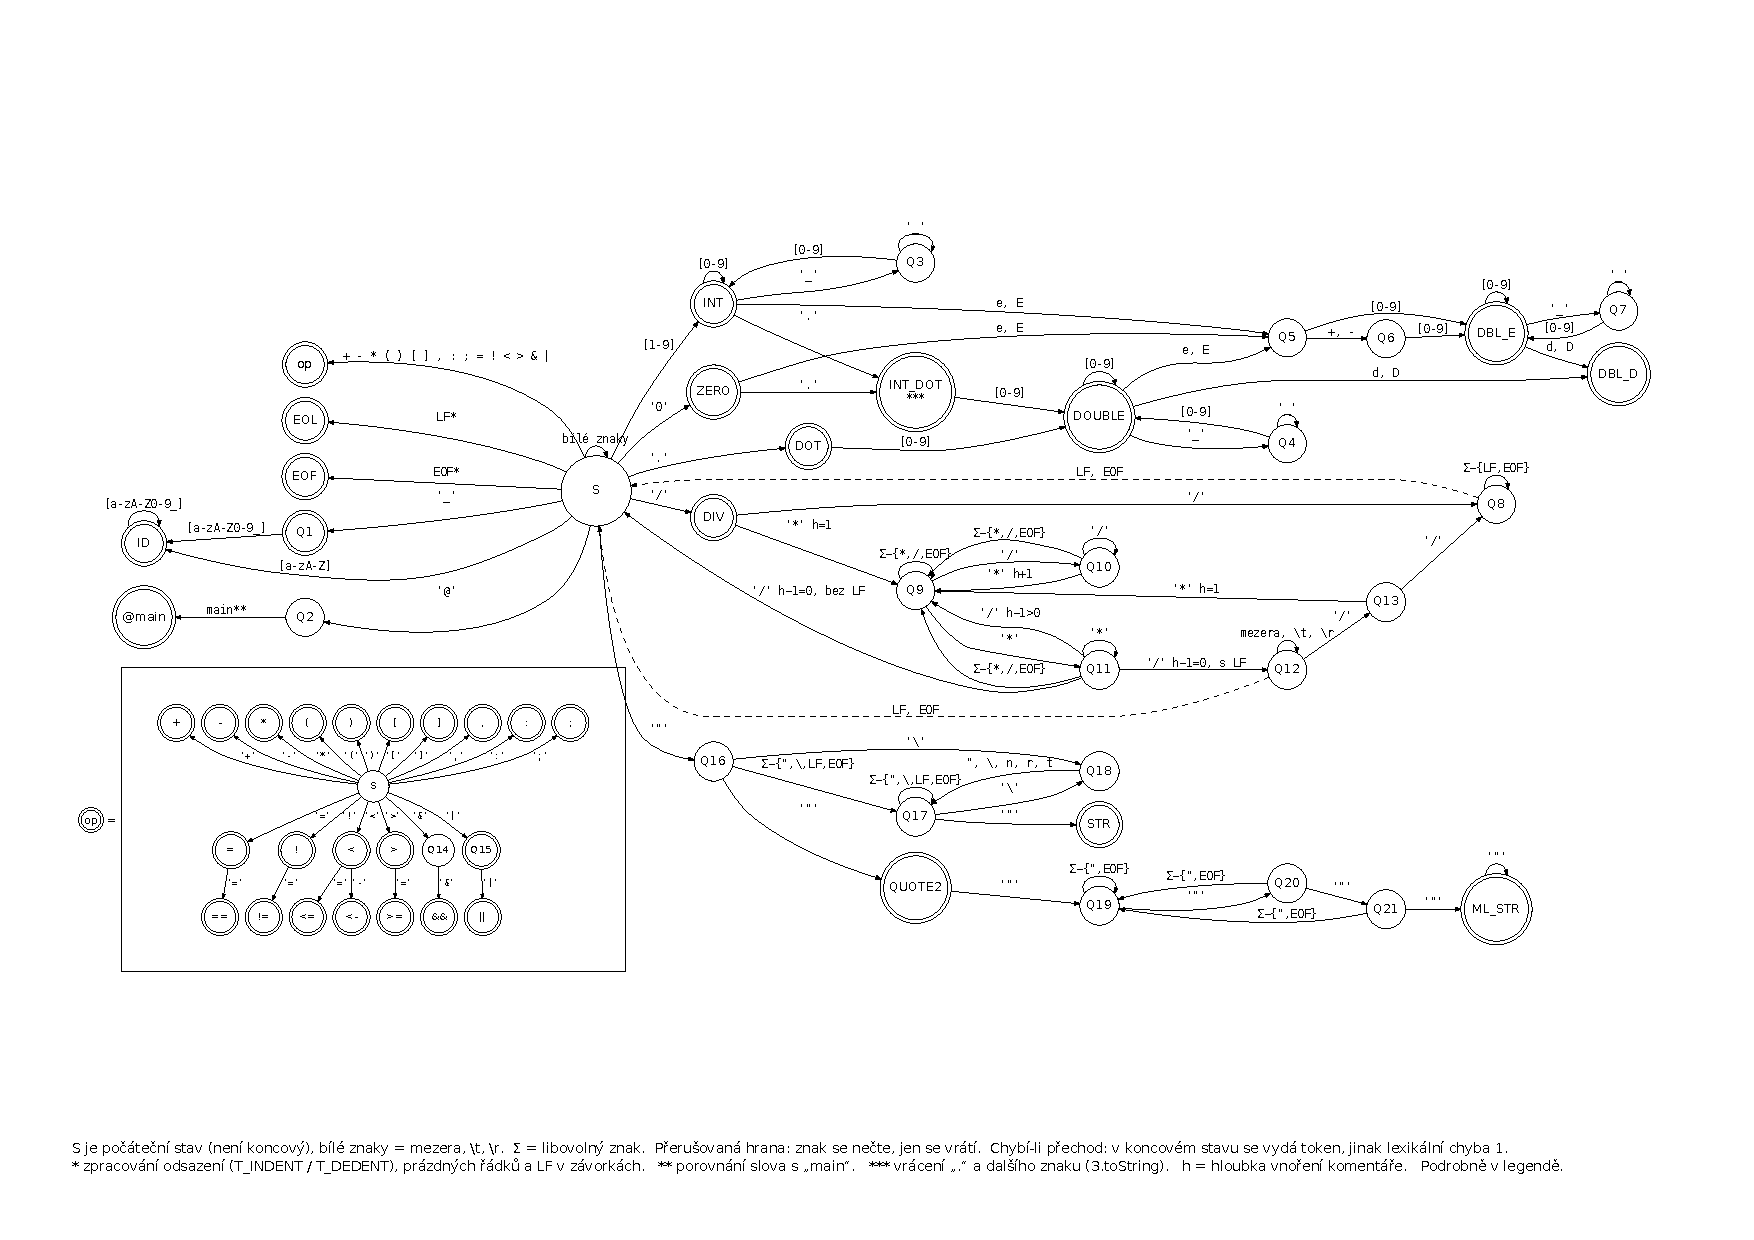
\includepdf[pages=-,fitpaper]{fsm.pdf}

\end{document}